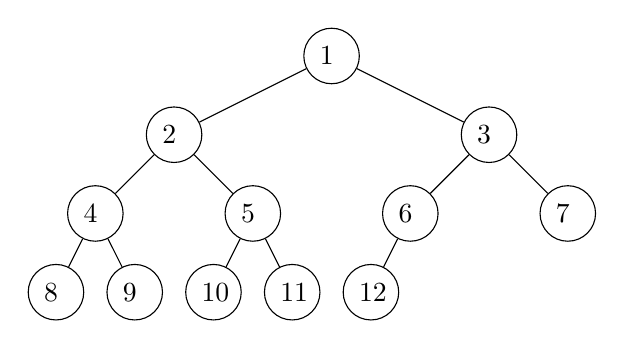
\begin{tikzpicture}[level distance=10mm]
  \tikzstyle{every node}=[circle,draw,text width=0.3cm]
  \tikzstyle{level 1}=[sibling distance=4cm]
  \tikzstyle{level 2}=[sibling distance=2cm]
  \tikzstyle{level 3}=[sibling distance=1cm]
  \node {1}
  child {node {2}
    child {node {4}
      child {node {8}}
      child {node {9}}
    }
    child {node {5}
      child {node {10}}
      child {node {11}}
    }
  }
  child {node {3}
    child {node {6}
      child {node {12}}
      child[fill=none] {edge from parent[draw=none]}
    }
    child {node {7}}
  };
\end{tikzpicture}
